\chapter{Введение в байесовские методы} 
\section{Основные определения.}
Вероятность на $\Omega$ с $\sigma$-алгеброй $\mathscr{A}$ --- это отображение $P: \mathscr{A} \rightarrow \mathbb{R}$, удовлетворяющая следующим аксиомам:
\begin{enumerate}
	\item неотрицательность: $P(A) \geq 0, \quad \forall A \in \mathscr{A}$
	\item нормированность: $P(\Omega)=1$
	\item аддитивность: $P(A \cup B) = P(A) + P(B), \quad A \bigcap B = \emptyset$
	\item непрерывность в нуле: $\forall B_1 \supset B_2 \supset B_3 \supset \dots \quad \text{и} \quad \bigcap\limits_{i=1}^{\infty} B_i = \emptyset \Rightarrow \\ P(B_n)\xrightarrow[n \to 0]{} 0$
\end{enumerate}
тогда $(\Omega, \mathscr{A}, P)$  --- вероятностное пространство.

Две случайные величины называются независимыми, если:
$$P(A \cap B) = P(A) P(B)$$

Вероятность события $B$ при условии свершения события $A$ называется условной, если:
$$P(B \arrowvert A) = \frac{P(B \cap A)}{P(A)}, \quad P(A) > 0, 
$$
$$
(\Omega, \mathscr{A}, P) \text{--- вероятностное пространство.}
$$

Исходя из определения условной вероятности следует цепное правило:
\begin{itemize}
	\item $P(X \cap Y) = P(B \arrowvert A) P(A)$
	\item $P(X \cap Y \cap Z) = P(X \arrowvert Y \cap Z) P(Y \arrowvert Z) P(Z)$
	\item $P(X_1 \cap \dots \cap X_n) = \prod\limits_{i=1}^{N} P(X_i \arrowvert X_1, \dots, X_{i-1})$
\end{itemize}
А также правило суммы:
$$
	P(X) = \int\limits_{-\infty}^{\infty} P(X, Y) dY
$$
И, наконец, самая важная теорема данной работы --- теорема Байеса:

$
 \Theta \text{ -- параметры (например параметры модели),}
$

$
	X \text{ -- наблюдения (например некоторые данные), тогда}
$
$$
 P(\Theta \arrowvert X) = \frac{P(X \cap \Theta)}{P(X)} = \frac{P(X \arrowvert \Theta) P(\Theta)}{P(X)}
 \text{ , где:}
$$

$P(\Theta)$ -- априорная вероятность параметров $\Theta$ (начальные сведения (вероятность) о параметрах (исходя из распределения $\Theta$ ));


$P(\Theta \arrowvert X)$ -- апостериорная вероятность (начальные сведения (вероятность) о параметрах, после получения некоторых данных);


$P(X \arrowvert \Theta)$ -- правдоподобие (показывает насколько хорошо параметры интерпретируют наши данные);


$P(X)$ -- полная вероятность наступления события B.

Исходя из данной теоремы можно ввести понятие online обучения. Предполагая, что у нас есть данные, приходящие маленькими порциями, можно обновлять параметры модели и затем, используя новую апостериорную вероятность как априорную можно перейти к следующему эксперименту с новой порцией данных:
$$
 P_k(\Theta) = P(\Theta \arrowvert X_k) = \frac{P(X_k \arrowvert \Theta) P_{k-1}(\Theta)}{P(X_k)}
$$

Рассмотрим модель наивного байесовского классификатора. У нас есть значения класса $C$, которые прямо воздействует на значения из других классов $A_1, A_3, A_3, A_4$. При этом $A_1, A_2, A_3, A_4$  не влияют друг на друга и их распределение может быть различное, тогда совместное распределение  при помощи теоремы Байеса можно представить в виде:
$$
 P(C \cap A_1 \cap A_2 \cap A_3 \cap A_4) = P(C) \prod\limits_{i=1}^{4} P(A_i \arrowvert C)
$$

\begin{figure}[H]
	\center{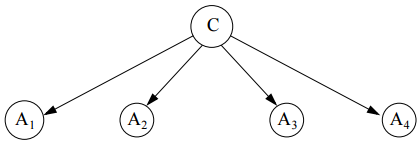
\includegraphics[width=0.7\linewidth]{pictures/naive_bayessian_classifier}}
	\caption{Наивный байесовский классификатор}
\end{figure}

Также введём понятие многомерного нормального распределения как:
$$
 \mathscr{N}(x \arrowvert \mu, \Sigma) = \frac{1}{\sqrt{|2 \pi \Sigma|}} \exp^{-\frac{1}{2}(x-\mu)^\top \Sigma^{-1} (x-\mu)}
 \text{ , где:}
$$
$\mathbb{E}X = \mu$ -- вектор средних значений (вектор мат. ожидания) \\
$Cov[X] = \Sigma$ -- матрица ковариации
%\begin{figure}[H]
%\centering
%\subfigure[Сверточный слой(5 нейронов)]{\label{fig:a}\includegraphics[width=0.5\linewidth]{depthcol}}
%\subfigure[Принцип работы pooling слоя]{\label{fig:b}\includegraphics[width=0.7\linewidth]{maxpool}}
%\subfigure[Полносвязный слой]{\label{fig:b}\includegraphics[width=0.7\linewidth]{photo_2018-05-27_21-18-01}}
%\caption{Типы слоев в сверточных нейросетях}
%\end{figure}

Представим таким же способом модель линейной регрессии. Есть три класса веса, данные и метки под данные. Тогда, с учётом того, что все распределения нормальные, имеем:
\begin{align*}
& P(w, y \arrowvert X) = P(y \arrowvert X, w) P(w) \\
& P(y \arrowvert w, X) = \mathscr{N}(y \arrowvert w^\top X, \sigma^2 I) \\
& P(w)=\mathscr{N}(y \arrowvert 0, \gamma^2 I) \\
\end{align*}

Тогда, исходя из данного представления, поставив задачу максимизации вероятности весов при условии предоставленных данных,  получим следующую задачу оптимизации $P(w \arrowvert y, X) \rightarrow \max\limits_{w}^{} $. Из которой можно получить:
$$
	\|y - w^\top X\|^2 + \underbrace{\lambda \|w\|^2}_{L_2 \text{ regualizer}} \rightarrow \max\limits_{w}^{}
$$

\begin{figure}[H]
	\center{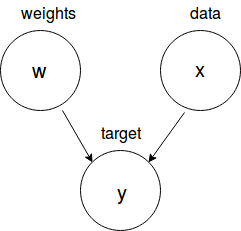
\includegraphics[width=0.4\linewidth]{pictures/linear_regression_model}}
	\caption{Модель линейной регрессии}
\end{figure}
\newpage

\section{Сопряжённое априорное распределение.}
Априорная вероятность $P(\Theta)$ называется сопряжённой его правдоподобию $P(X \arrowvert \Theta)$, если априорная вероятность $P(\Theta)$ и апостериорная $P(\Theta \arrowvert X)$ из одного семейства распределений.

Если априорная вероятность -- нормальная и параметризированна некоторыми параметрами $\mu$ и $\sigma$, то, чтобы она была сопряженной правдоподобию,z мы ожидаем, чтобы апостериорная вероятность была также нормальной, но с уже другими $\mu$ и $\sigma$.
Например, правдоподобие нормальное со средним $\Theta$ и дисперсией $\sigma^2$ . Если взять априорное распределнеие за нормальное, но с другими параметрами, то после перемножения и нормализацию на определённую константу, мы также получим нормальное распределение.  
$$
 \underbrace{P(\Theta \arrowvert X)}_{\mathscr{N}(y \arrowvert a, b^2)} = \frac{\overbrace{P(X \arrowvert \Theta)}^{\mathscr{N}(y \arrowvert \Theta, \sigma^2)} \overbrace{P(\Theta)}^{\mathscr{N}(\Theta \arrowvert m, s^2)}}{\underbrace{P(X)}_{\text{константа}}}
$$
Рассмотрим реальный пример. Представим, что правдоподобие нормальное со средним $\Theta$ и дисперсией 1 и априорное распределение является стандартным нормальным (среднее - 0, дисперсия - 1), тогда:
\begin{align*}
& p(\Theta \arrowvert x) = \frac{p(x \arrowvert \Theta) p(\Theta)}{p(x)} = \frac{\mathscr{N}(x \arrowvert \Theta, 1) \mathscr{N}(\Theta \arrowvert 0, 1)}{p(x)}\\
& p(\Theta \arrowvert x) \propto  e^{- \frac{1}{2} (x - \Theta)^2}  e^{- \frac{1}{2} \Theta^2} \\
& p(\Theta \arrowvert x) \propto  e^{-(\Theta - \frac{x}{2})^2} \\
& p(\Theta \arrowvert X) = \mathscr{N}(\Theta \arrowvert \frac{x}{2}, \frac{1}{2}) \\
\end{align*}
\chapter{EM-алгоритм}
\section{Модель скрытых переменных.}
EM-алгоритм - алгоритм, используемый в математической статистике для нахождения оценок максимального правдоподобия параметров вероятностных моделей, в случае, когда модель зависит от некоторых скрытых переменных. 
Как правило, ЕМ-алгоритм применяется для решения задач двух типов:
\begin{itemize}
	\item К первому типу можно отнести задачи, связанные с анализом действительно неполных данных, когда некоторые статистические данные отсутствуют в силу каких-либо причин.
	\item Ко второму типу задач можно отнести те задачи, в которых функция правдоподобия имеет вид, не допускающий удобных аналитических методов исследования, но допускающий серьезные упрощения, если в задачу ввести дополнительные «ненаблюдаемые» (скрытые, латентные) переменные. Примерами прикладных задач второго типа являются задачи распознавания образов, реконструкции изображений. Математическую суть данных задач составляют задачи кластерного анализа, классификации и разделения смесей вероятностных распределений.
\end{itemize}

На передовых рубежах глубокого обучения часто требуется построить вероятностную модель входа, $p_{\text{model}} (x)$. В принципе, в такой модели может использоваться вероятностный вывод для предсказания любой переменной в ее окружении при известных других переменных. Во многих моделях имеются также латентные переменные $h$, так что $p_{\text{model}}(x) = \mathbb{E}_{h} p_{\text{model}}(x \arrowvert h)$. Латентные переменные дают еще один способ представления данных. Распределенные представления, основанные на латентных переменных, могут пользоваться всеми преимуществами обучения представлений.
Предположим, что в данных есть латентные переменные (скрытые переменные, скрытые компоненты), причем модель устроена так, что если бы мы их знали, задача стала бы проще, а то и допускала бы аналитическое решение. На самом деле, совершенно не обязательно, чтобы эти переменные имели какой-то физический смысл, может быть, так просто удобнее, но физический смысл (такой, как номер кластера в предыдущем примере), конечно, обычно помогает их придумать. Например, задача порождения картинок с изображением цифр. В данной задаче необходимо породить всю картинку целиком так, чтобы она была «посвящена» одной и той же цифре, ведь половина двойки и половина восьмерки дадут скорее что-то похожее на рукописный твердый знак, чем на конкретную цифру. И это удобнее всего выразить именно так: сначала мы порождаем скрытую переменную z, которая соответствует тому, какую цифру хочется породить, а потом все распределение видимых данных $p(x \arrowvert z)$ будет уже зависеть от значения $z$.

\section{EM-алгоритм}
Чтобы применить  методы к нейронным сетям, сначала нужно выяснить, как работают байесовские методы. Исходя из того, что рассмотрим байесовское обоснование для одного из основных методов классического обучения без учителя, алгоритм  Expectation -- Maximization, который обычно называют просто EM-алгоритмом.

Идея EM-алгоритма довольно проста. Например, задача кластеризации на обычной плоскости $\mathbb{R}^2$: существует множество точек, необходимо разбить их на подмножества так, чтобы внутри каждой из них точки были «похожи» друг на друга, то есть они близки друг к другу, и точки из разных подмножеств могли бы быть значительно более различны, то есть находились бы далеко на плоскости.

Предположим, что существует вероятностная модель, определяемая совместным распределением $p(X, T \arrowvert \Theta)$. Здесь $X$ -- набор наблюдаемых переменных, $T$ -- набор ненаблюдаемых переменных и $\Theta$ -- набор параметров модели. Рассмотрим проблему изучения модели (поиск параметров Ө по образцу X) с использованием метода максимального правдоподобия:
\begin{equation}  \label{eq:one}
 \log{p(X \arrowvert \Theta)} = \log{\int{p(X,T \arrowvert \Theta) dT} \rightarrow \max\limits_{\Theta}^{} }
\end{equation}

Рассмотрим произвольное вероятностное распределение $q(T)$. Тогда справедлива следующая цепочка равенств:

\begin{align*} 
 &\log{p(X \arrowvert \Theta)} = \int{q(T) \log{p(X \arrowvert \Theta)} dT} = \int{q(T) \log{\frac{p(X,T \arrowvert \Theta)}{p(T \arrowvert X, \Theta)}} dT} =\\ & =\int{q(T) \log{  \bigg[ \frac{p(X,T \arrowvert \Theta)}{q(T)} \frac{q(T)}{p(T \arrowvert X, \Theta)}  \bigg] } dT} =  \\ 
 &=  \underbrace{\int{q(T) \log{p(X,T \arrowvert \Theta)} dT} - \int{q(T) \log{q(T)} dT}}_{\mathcal{L}(q)} - \underbrace{\int{q(T) \log{\frac{p(T \arrowvert X, \Theta)}{q(T)}} dT}}_{KL(q \| p(T \arrowvert X, \Theta) )}
\end{align*}

Дивергенция $KL(q \| p(T \arrowvert X, \Theta) ) \geq 0$, следовательно:
\begin{equation} \label{eq:two}
	\log{p(X \arrowvert \Theta)} \geq \mathcal{L}(q)
\end{equation}

EM-алгоритм для решения задачи \eqref{eq:one} является аналогом метода Ньютона для оптимизации произвольной функции, где вместо квадратичного приближения в текущей точке используется нижняя оценка \eqref{eq:two}. Пусть некоторое значение параметров $\Theta_{\text{old}}$ будет фиксированным. Сначала (на шаге E) определяется распределение $q(T)$ как распределение значений скрытых переменных с заданными параметрами:
\begin{equation} \label{eq:three}
	q(T) = p(T \arrowvert X, \Theta_{\text{old}}) = \frac{p(X, T \arrowvert \Theta_{\text{old}})}{\int{p(X, T \arrowvert \Theta_{\text{old}}) dT}}
\end{equation}

При таком выборе $q(T)$ нижняя оценка \eqref{eq:two} является точной для $\Theta = \Theta_{\text{old}}$. Затем (на М-шаге) новые значения параметров находят путем максимизации нижней границы $\mathcal{L}(q)$, что эквивалентно решению задачи:
\begin{equation} \label{eq:four}
 \mathbb{E}_{T \arrowvert X,  \Theta_{\text{old}}}\log{p(X, T \arrowvert \Theta)} \rightarrow \max\limits_{\Theta}^{}
\end{equation}
так как энтропия -- $\mathbb{E}_q \log{q(T)}$ распределения $q(T)$ не зависит от $\Theta$. Шаги Е и М повторяются в цикле до сходимости. Очевидно, что в процессе ЕМ-итераций нижняя оценка \eqref{eq:two}, а также значение правдоподобия $p(X| \Theta)$ не убывают. Монотонное неубывание правдоподобия $p(X|\Theta)$ и его ограниченность сверху гарантируют общую сходимость ЕМ-итераций.

Итерационный процесс в ЕМ-алгоритме проиллюстрирован на рисунке \ref{fig:three}. Нижняя оценка \eqref{eq:two} обозначена через $\mathcal{L}(q, \Theta)$. По аналогии со многими итерационными методами оптимизации, ЕМ-алгоритм позволяет находить только локальный максимум правдоподобия.
\begin{figure}[H]
	\center{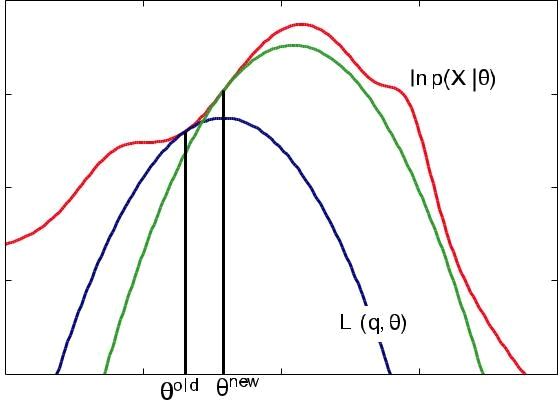
\includegraphics[width=0.7\linewidth]{pictures/iter_process}}
	\caption{Итерационный процесс в EM-алгоритме }
	\label{fig:three}
\end{figure}
Заметим, что во многих практических случаях решение задачи \ref{eq:four} намного проще, чем решение задачи \ref{eq:one}. В частности, в рассматриваемой ниже задаче разделения гауссовской смеси задача оптимизации на М шаге может быть решена аналитически.   
      
Вычисление значения функции правдоподобия $p(X \arrowvert \Theta)$ в фиксированной точке требует интегрирования по пространству $T$ и в ряде случаев может представлять собой вычислительно трудоемкую задачу. Заметим, что эта величина правдоподобия необходима также для вычисления апостериорного распределения $p(T \arrowvert X, \Theta_{\text{old}})$ на Е-шаге. Однако, распределение $p(T \arrowvert X, \Theta_{\text{old}})$ используется затем только для вычисления математического ожидания логарифма полного правдоподобия на М-шаге. Как правило, здесь не требуется знать все апостериорное распределение целиком, а достаточно знать лишь несколько статистик этого распределения (например, только мат.ожидания отдельных компонент $\mathbb{E}_{T \arrowvert X, \Theta_{\text{old}} t_n}$ и парные ковариации $\mathbb{E}_{T \arrowvert X, \Theta_{\text{old}} t_n t_k}$). Поэтому ЕМ-алгоритм может быть вычислительно эффективен даже в тех случаях, когда вычисление значения правдоподобия $p(X \arrowvert \Theta)$ в одной точке затруднено.
                  
EM-алгоритм можно рассматривать как подъем по координатам для максимизации нижней границы \ref{eq:two}. Сначала при фиксированных параметрах $\Theta_{\text{old}}$ нижняя граница максимизируется по распределению $q(T)$ (эта задача имеет аналитическое решение $q(T) = p(T \arrowvert X,  \Theta_{\text{old}})$). Затем для фиксированного $q(T)$ нижняя граница максимизируется по параметрам. Если апостериорное распределение $p(T \arrowvert X, \Theta_{\text{old}})$ не может быть вычислено, то мы можем ограничить семейство распределений $q(T)$ параметрическим или факторизованным семейством и решить задачу максимизации нижней границы в пределах выбранного семейства распределений. В этом случае будет обеспечен монотонный рост нижнего предела правдоподобия, но, вообще говоря, не самого значения правдоподобия $p(X \arrowvert \Theta)$. В случае невозможности точного решения задачи на шаге M можно ограничиться только движением в направлении увеличения нижней границы.\cite{em}
          
ЕМ-алгоритм можно применять также для решения задачи обучения вероятностной модели со скрытыми переменными $p(X, T \arrowvert \Theta )$ с помощью максимизации апостериорного распределения:
$$
p(\Theta \arrowvert X) \rightarrow \max\limits_{\Theta}^{} \Leftrightarrow \log{p(X \arrowvert \Theta)} + \log{p(\Theta)} \rightarrow \max\limits_{\Theta}^{}
$$

Здесь $p(\Theta)$ — априорное распределение на параметры модели. В этом случае нижней оценкой для оптимизируемого функционала является следующая величина:
$$
 \log{p(X \arrowvert \Theta)} + \log{p(\Theta)} \geq \mathcal{L}(q) + \log{p(\Theta)}
$$

Итерационная оптимизация данной нижней границы по распределению $q(T)$ и по параметрам приводит к Е-шагу \ref{eq:three} и М шагу:
$$
 \mathbb{E}_{T \arrowvert X,  \Theta_{\text{old}}}\log{p(X, T \arrowvert \Theta)} + \log{p(\Theta)} \rightarrow \max\limits_{\Theta}^{}
$$
\section{Применение и примеры EM-алгоритма}

Рассмотрим вероятностную модель смеси нормальных распределений:

\begin{equation} \label{eq:five}
 p(x) = \sum\limits_{k=1}^{K} \omega_k \mathcal{N}(x \arrowvert \mu_k,  \Sigma_k), \quad \sum\limits_{k=1}^{K} \omega_k = 1, \quad \omega_k \geq 0 
\end{equation}

Модель смеси распределений (не обязательно нормальных) можно рассматривать как модель со скрытой переменной t, которая обозначает номер компоненты смеси:

\begin{align}
p(t=k) &= \omega_k \label{eq:six}\\
p(x \arrowvert t = k) &= \mathcal{N}(x \arrowvert \mu_k, \Sigma_k) \label{eq:seven}
\end{align}

Легко показать, что маргинальное распределение $p(x) = \sum_k p(x \arrowvert t = k)p(t = k)$ в этой модели совпадает с распределением \ref{eq:five}. В этом смысле модели \ref{eq:six} -- \ref{eq:seven} и \ref{eq:five} эквивалентны.
Интерпретация вероятностной модели смеси распределений как модели со скрытой переменной позволяет генерировать выборку из модели смеси следующим образом. Сначала с вероятностями, равными $\omega$, генерируется номер компоненты смеси, из которой затем генерируется точка $x$.

Для аппроксимации выборки $X = \{x_1, \dots , x_N \}$ с помощью модели смеси из $K$ гауссиан можно воспользоваться методом максимального правдоподобия:

\begin{equation} 
	\begin{array}{r@{}l} \label{eq:eight}
		 p(X \arrowvert \omega, {\mu_k}, {\Sigma_k}) &{}= \prod_{n=1}^{N} p(X \arrowvert \omega, {\mu_k}, {\Sigma_k}) \\ &{}= \prod_{n=1}^{N} \Big ( \sum\limits_{K}^{} \omega_k \mathcal{N}(x_n \arrowvert \mu_k, \Sigma_k) \Big ) \rightarrow \max\limits_{\omega, {\mu_k}, {\Sigma_k}}^{}, \\
		 &{}\sum\limits_{k=1}^{K} \omega_k = 1, \quad \omega_k \geq 0 \\
		 &{}\sum_{K} = \sum\limits_{K}^{T}, \quad \sum_{K} \succ 0
	\end{array}{}
\end{equation}

Данная проблема условной оптимизации может быть эффективно решена с использованием EM-алгоритма, описанного в предыдущем подразделе. Стоит обратить внимание, что число компонентов смеси $K$ не может быть найдено аналогичным образом путем максимизации вероятности, поскольку значение вероятности данных тем выше, чем больше используется компонент $K$. Чтобы найти оптимальное значение $K$, можно использовать кросс-валидацию, где критерием качества аппроксимации тестовых данных является значение правдоподобия. \cite{em}
При использовании ЕМ-алгоритма для решения задачи \ref{eq:eight} вероятностная модель смеси распределений интерпретируется как вероятностная модель со скрытыми переменными. Вычислим значение математическое ожидание логарифма полного правдоподобия, необходимого для решения задачи оптимизации на М шаге:


\begin{equation} \label{eq:nine}
	\mathbb{E}_{q}\log{p(X, T \arrowvert \omega,  \{\mu_k\}, \{\Sigma_k\})} = \sum\limits_{n=1}^{N} \sum\limits_{k=1}^{K} q(t_n=k)(\log{\omega_k} + \log{\mathcal{N}(x_n \arrowvert \mu_k, \Sigma_k)})
\end{equation}

Выражение зависит только от вероятностей отдельных скрытых переменных $q(t_n = k)$. Эти величины можно найти следующим образом:

\begin{equation} 
	\begin{array}{r@{}l} \label{eq:ten}
		 \gamma_{nk} \coloneqq q(t_n = k) &{}= p(t_n=k \arrowvert x_n, \omega^{\text{old}}, \{\mu_k^{\text{old}}\},  \{\Sigma_k^{\text{old}}\}) = \\ 
		 &{}= \frac{\omega_k^{\text{old}} \mathcal{N}(x_n \arrowvert \mu_k^{\text{old}}, \Sigma_k^{\text{old}})}{\sum_{j=1}^{K} \omega_j^{\text{old}} \mathcal{N}(x_n \arrowvert \mu_j^{\text{old}}, \Sigma_j^{\text{old}})}
	\end{array}{}
\end{equation}

Задача максимизации критерия \ref{eq:ten} при ограничениях $\sum_{k=1}^K \omega_k = 1$, $w_k \geq 0$ может быть решена аналитически:

\begin{align}
\omega_k &= \frac{1}{N} \sum_{n=1}^{N} \gamma_{nk} \label{eq:eleven} \\
\mu_k &= \frac{\sum_{n=1}^{N} \gamma_{nk} x_n}{\sum_{n=1}^{N} \gamma_{nk}} \label{eq:twelve}\\
\Sigma_k &= \frac{\sum_{n=1}^{N} \gamma_{nk} (x_n-\mu_k)(x_n-\mu_k)^\top}{\sum_{n=1}^{N} \gamma_{nk}} \label{eq:13}
\end{align}

Решение для $\sum_{K}^{}$ \ref{eq:13} удовлетворяет условию симметричности и положительной определенности. Кроме того, формулы \ref{eq:twelve}, \ref{eq:13} соответствуют оценкам максимального правдоподобия для многомерного нормального распределения, в которых каждый объект $x_n$ берется с весом $\gamma_{nk}$.

Таким образом, ЕМ-алгоритм для смеси нормальных распределений заключается в итерационном применении формул \ref{eq:ten} и \ref{eq:eleven}-\ref{eq:13}. Этот процесс имеет простую интерпретацию. Величина $\gamma_{nk}$ показывает степень соответствия между объектом $x_n$ и компонентой $k$ (определяет вес объекта $x_n$ для компоненты $k$). Эти веса затем используются на М шаге для вычисления новых значений параметров компонент. Пример применения ЕМ-алгоритма для разделения нормальной смеси с двумя компонентами показана на рисунке 2.2. На рисунке \ref{fig:a} показана исходная выборка и     начальное приближение для двух компонент. На рисунке \ref{fig:b} показан результат Е шага, при     этом цвета объектов соответствуют     значениям $\gamma_{nk}$.     На рисунках \ref{fig:c} -- \ref{fig:f} показаны результаты вычислений после 1, 2, 5 и 20 итераций. \cite{em}

\begin{figure}[H]
	\centering
	\label{fig:A}
	\subfigure[]{\label{fig:a}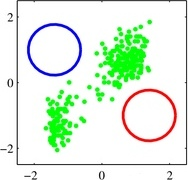
\includegraphics[width=0.3\linewidth]{pictures/gmm_1}} 
	\subfigure[]{\label{fig:b}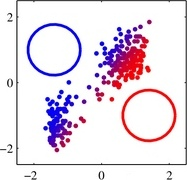
\includegraphics[width=0.3\linewidth]{pictures/gmm_2}} %\label{fig:4_2}
	\subfigure[]{\label{fig:c}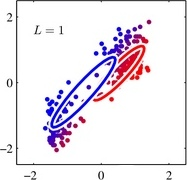
\includegraphics[width=0.3\linewidth]{pictures/gmm_3}} %\label{fig:4_3}
	\subfigure[]{\label{fig:d}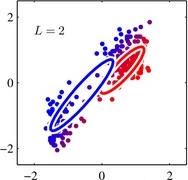
\includegraphics[width=0.3\linewidth]{pictures/gmm_4}} %\label{fig:4_4}
	\subfigure[]{\label{fig:e}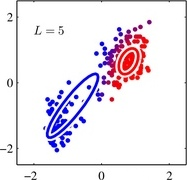
\includegraphics[width=0.3\linewidth]{pictures/gmm_5}} %\label{fig:4_5}
	\subfigure[]{\label{fig:f}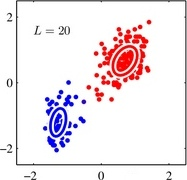
\includegraphics[width=0.3\linewidth]{pictures/gmm_6}} %\label{fig:4_6}
	\caption{Применения ЕМ-алгоритма для разделения нормальной смеси}
\end{figure}

Одним из применений смеси нормальных распределений является решение задачи кластеризации на $K$ кластеров. В этом случае номер кластера для объекта $x_n$ определяется величиной:

$$
	k_n = \arg \max_k \gamma_{nk}
$$

Такая схема кластеризации является вероятностным обобщением известного метода кластеризации $K$-средних.
В заключение этого раздела заметим, что восстановление плотности по данным (в частности, смеси нормальных распределений) является  простейшим способом решения задачи идентификации. Для этого сначала для всех объектов обучающей выборки, обладающих заданным свойством, восстанавливается плотность распределения. Затем, для нового объекта $x$ решение о наличии у него заданного свойства принимается, если значение восстановленной плотности $p(x)$ выше определенного порога.

\chapter{Вариационные автокодировщики}
\section{Введение в вариационные автокодировщики}
Глубокие сверточные нейронные сети (CNN) используются на данный момент для достижения самого лучшего качества во многих задачах компьютерного зрения с учителем, таких как классификация изображений, поиск, детекция и восстановление. Глубокие генеративные модели на основе CNN, ветвь методов обучения без учителя в машинном обучении, стали горячей темой исследований в области компьютерного зрения в последние годы. Генеративная модель, обученная с данным набором данных, может использоваться для генерации данных, имеющих свойства, аналогичные образцам в наборе данных, для изучения внутренней сущности набора данных и «хранения» всей информации в ограниченных параметрах, которые значительно меньше, чем обучающий набор данных.

Вариационный автокадировщик Variational Autoencoder (VAE) стал популярной порождающей моделью, что позволяет формализовать проблему в рамках вероятностных графических моделей со скрытыми переменными. По умолчанию для измерения разницы между восстановленными и исходными изображениями используется измерение по пикселям, например функция потерь $L_2$ или функция потерь логистической регрессии. Такие измерения легко осуществимы и эффективны для глубокого обучения нейронной сети. Однако сгенерированные изображения имеют тенденцию быть очень размытыми по сравнению с естественными изображениями. Это связано с тем, что потери по пикселям не отражают разницу в восприятии и пространственную корреляцию между двумя изображениями. Например, одно и то же изображение, смещенное на несколько пикселей, будет иметь незначительное визуальное восприятие для людей, но оно может иметь очень высокую попиксельную функцию потерь. Это хорошо известная проблема в сообществе по измерению качества изображения.

Из литературы по измерению качества изображения известно, что потеря пространственной корреляции является основным фактором, влияющим на визуальное качество изображения. Недавние работы по синтезу текстур и передаче стиля показали, что скрытые представления глубокой CNN могут захватывать различные свойства пространственной корреляции входного изображения. Воспользуемся этим свойством CNN и пытаемся улучшить VAE, заменив попиксельную потерю на потерю восприятия объекта, которая определяется как разница между скрытыми представлениями двух изображений, извлеченными из предварительно обученной глубокой CNN, такой как AlexNet и VGGNet прошли обучение по ImageNet. Основная идея состоит в том, чтобы попытаться улучшить качество генерируемых изображений VAE путем обеспечения согласованности скрытых представлений входного и выходного изображений, что, в свою очередь, налагает пространственную корреляционную согласованность двух изображений. Также будет показано, что скрытые векторы AVE, обученные с помощью данного метода, обладают мощной концептуальной способностью представления и могут использоваться для достижения самых современных характеристик в прогнозировании характеристик лица.

VAE помогает делать две вещи. Во-первых, это позволяет кодировать изображение $x$ в скрытый вектор $z = \text{Encoder}(x) \sim q(z \arrowvert x)$ с помощью сети кодера, а затем сеть декодера используется для декодирования скрытого вектора $z$ обратно в изображение, которое будет таким же, как исходное изображение $\overline{x} = \text{Decoder}(z) \sim p (x \arrowvert z)$. То есть нам нужно максимизировать предельную логарифмическую вероятность каждого наблюдения (пикселя) в $x$, а потери реконструкции VAE $\mathcal{L}_{\text{rec}}$ - это отрицательная ожидаемая логарифмическая вероятность наблюдений в $x$. Другим важным свойством VAE является способность управлять распределением скрытого вектора $z$, который имеет характерную независимость от единичных гауссовских случайных величин, то есть $z \sim \mathcal{N}(0, I)$. Кроме того, различие между распределением $q(z \arrowvert x)$ и распределением Гаусса (называемое расходимостью дивергенции кульбака-лейблера ($KL$)) может быть количественно оценено и минимизировано с помощью алгоритма градиентного спуска. Следовательно, модели VAE можно обучать путем оптимизации суммы потерь на восстановление ($\mathcal{L}_{\text{rec}}$) и потерь на расхождение дивергенции кульбака-лейблера ($\mathcal{L}_{\text{kl}}$) путем градиентного спуска.

\begin{align}
\mathcal{L}_{\text{rec}} &{}= -\mathbb{E}_{q(z \arrowvert x)} \big[ \log{p(x \arrowvert z)} \big]\label{eq:14} \\ \nonumber \\
\mathcal{L}_{\text{kl}} &{}= D_{\text{kl}}(q(z \arrowvert x) \| p(z)) \label{eq:15}\\ \nonumber \\
\mathcal{L}_{\text{vae}} &{}=\mathcal{L}_{\text{rec}} + \mathcal{L}_{\text{kl}} \label{eq:16}
\end{align}

Были предложены другие методы для улучшения производительности VAE. Например можно расширить вариационные автокодеры до полууправляемого обучения с помощью меток классов. Другой метод предлагает разнообразные условно-зависимые глубокие вариационные автокодеры и демонстрирует, что они способны генерировать реалистичные лица с разнообразным внешним видом, Deep Recurrent Attentive Writer (DRAW) сочетает в себе механизм пространственного внимания с последовательной вариационной структурой автокодирования, которая позволяет повторять генерацию изображений. Принимая во внимание недостаток попиксельной потери, заменить ее на многомасштабную оценку структурного сходства (MS-SSIM) и демонстрирует, что он может лучше измерять восприятие качества изображения. Также можно усилить целевую функцию дискриминационной регуляризацией. Еще один подход пытается объединить VAE и порождающую состязательную сеть (GAN) и использовать представление изученных признаков в дискриминаторе GAN в качестве основы для цели реконструкции VAE.
\section{Высокоуровневая пространственная функция потерь \\ (perceptrual loss)}

Несколько недавних работ успешно генерируют изображения путем оптимизации потери восприятия, которая основана на высокоуровневых функциях, извлеченных из предварительно обученных глубоких CNN. Передача нейронного стиля и синтез текстуры пытаются совместно минимизировать потери при восстановлении элементов высокого уровня и потери при реконструкции стиля путем оптимизации. Кроме того, изображения могут быть также получены путем максимизации оценки классификации или отдельных функций. В других работах делается попытка обучить сеть прямой распространения для передачи в режиме реального времени и сверхразрешения на основе потери восприятия функции. В данной главе будет обучаться глубокий сверточный вариационный автокодировщик для генерации изображения, заменяя потерю реконструкции пиксель за пикселем потерей восприятия функции, основанной на предварительно обученной глубокой CNN.

Пространственная функция потерь признаков двух изображений определяется как разница между скрытыми признаками в предварительно обученной глубокой сверточной нейронной сети. Будем использовать VGGNet в качестве сети потерь в эксперименте, который обучен решению задачи классификации в наборе данных ImageNet. Основная идея пространственная функция потерь заключается в поиске согласованности между скрытыми представлениями двух изображений. Поскольку скрытые представления могут охватывать важные характеристики воспринимаемого качества, такие как пространственная корреляция, меньшая разница скрытых представлений указывает на согласованность пространственных корреляций между входом и выходом, в результате мы можем получить лучшее визуальное качество выходного изображения. В частности, пусть $\Phi(x)^l$ представляет вид $l$-го скрытого слоя, когда входное изображение $x$ подается в сеть $\Phi$. Математически $\Phi(x)$ l - массив трехмерных блоков формы $[C^l \times W^l \times H^l]$, где $C^l$ - количество фильтров, $W^l$ и $H^l$ - ширина и высота каждой карты объектов для $l$-го слоя соответственно. Потеря восприятия для одного слоя ($l$) между двумя изображениями $x$ и $\overline{x}$ может быть просто определена квадратом евклидова расстояния. На самом деле это очень похоже на попиксельную функция потерь, за исключением того, что цветовой канал не равен больше 3.
$$
 \mathcal{L}_{\text{rec}}^{l} = \frac{1}{2 C^l W^l H^l} \sum\limits_{c=1}^{C^l} \sum\limits_{c=1}^{W^l} \sum\limits_{c=1}^{H^l} (\Phi(x)_{\text{c,w,h}}^{l} - \Phi(\overline{x})_{\text{c,w,h}}^{l})^2
$$

Конечные потери при восстановлении определяются как общие потери путем объединения различных уровней сети VGG, $ \mathcal{L}_{\text{rec}} = \sum_{l} \mathcal{L}_{\text{rec}}^l$. Кроме того, мы принимаем потери дивергенции кульбака-лейблера $\mathcal{L}_{\text{kl}}$, чтобы регулеризировать сеть кодировщиков для управления распределением скрытой переменной $z$. Чтобы обучить VAE, мы совместно минимизируем потерю дивергенции KL $\mathcal{L}_{\text{kl}}$ и потерю восприятия $\mathcal{L}_{\text{rec}}^{l}$ для разных слоев.

$$
 \mathcal{L}_{\text{total}} = \alpha \mathcal{L}_{\text{kl}} + \beta \sum\limits_{i}^{l} \mathcal{L}_{\text{rec}}^l
$$
где $\alpha$ и $\beta$ - весовые параметры для дивергенции KL и восстановления изображения. Это очень похоже на передачу стиля, если мы рассматриваем дивергенцию кульбака-лейблера как реконструкцию стиля.

\section{Детали модели автокодировщика}

Разрабатываемая система состоит из двух основных компонентов, как показано на рисунке \ref{fig:autoencoder}: сеть автокодера, включающая в себя сеть $E(x)$ кодера и сеть $D(z)$ декодера, и сеть потерь $\Phi$, которая является предварительно обученной глубокой CNN для определения характеристики восприятия потери. Входное изображение $x$ кодируется как скрытый вектор $z=E(x)$, который будет декодирован обратно в пространство изображения $\overline{x}= D(z)$. После обучения сетью декодеров может быть сгенерировано новое изображение с заданным вектором $z$. 
 \begin{figure}[H]
 	\center{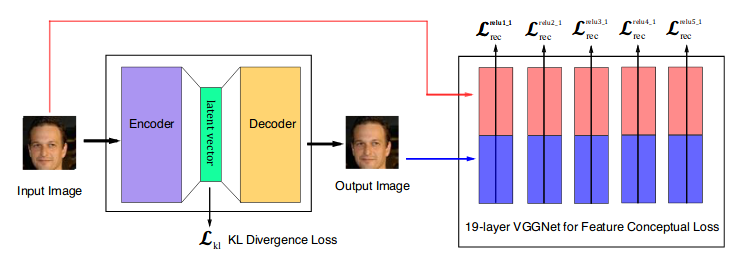
\includegraphics[width=0.9\linewidth]{pictures/architecture}}
 	\caption{Модель автоколировщика}
 	\label{fig:autoencoder}
 \end{figure}

Чтобы обучить VAE, нам нужны две потери, одна из которых - потеря дивергенции кульбака-лейблера $\mathcal{L}_{\text{kl}} = D_{\text{kl}} (q (zx) \| p(z))$, которая используется для того, чтобы убедиться, что скрытый вектор $z$ является независимой единицей случайной переменной Гаусса. Другая особенность - пространственная потеря. Вместо того, чтобы непосредственно сравнивать входное изображение и сгенерированное изображение в пиксельном пространстве, мы подаем их обоих на предварительно обученную глубокую CNN $\Phi$ соответственно и затем измеряем разницу между представлениями скрытого слоя, то есть $\mathcal{L}_{\text{rec}} = \mathcal{L}^1 + \mathcal{L}^2 + \dots + \mathcal{L}^l$, где $\mathcal{L}_l$ представляет потерю объекта на $l$-м скрытом слое. Таким образом, мы используем потерю признаков высокого уровня, чтобы лучше измерить воспринимаемые и семантические различия между двумя изображениями, потому что предварительно обученная сеть по классификации изображений уже включила воспринимаемую и семантическую информацию, которую мы желали. Во время обучения сеть с предварительно подготовленными потерями является фиксированной и предназначена только для высокоуровневого извлечения признаков, а потеря дивергенции кульбака-лейблера $\mathcal{L}_{\text{kl}}$ используется для обновления сети кодера, в то время как функция потери восприятия функции отвечает за обновление параметров как кодера, так и декодер.

Сеть кодера и декодера основана на глубокой CNN, такой как VGGNet. Создадим 4 сверточных слоя в сети кодера с $4 \times 4$ ядрами, и шаг фиксируется равным 2 для достижения пространственной понижающей дискретизации вместо использования детерминированных пространственных функций, таких как maxpooling. Каждый сверточный слой сопровождается слоем batch normalization и слоем активации LeakyReLU. Затем два полностью связанных выходных слоя (для среднего значения и дисперсии) добавляются в кодировщик и будут использоваться для вычисления потерь на дивергенцию кульбака-лейблера и выборки скрытой переменной $z$. Для декодера мы используем 4 сверточных слоя с ядрами $3 \times 3$ и устанавливаем шаг равным 1, а стандартное заполнение нулями заменяем заполнением репликации, то есть карта объектов ввода дополняется репликацией границы входа. Также используется batch normalizationи, чтобы помочь стабилизировать обучение и используем LeakyReLU в качестве функции активации. Детали архитектуры автоэнкодера показаны на рисунке \ref{fig:detail}.

 \begin{figure}[H]
	\center{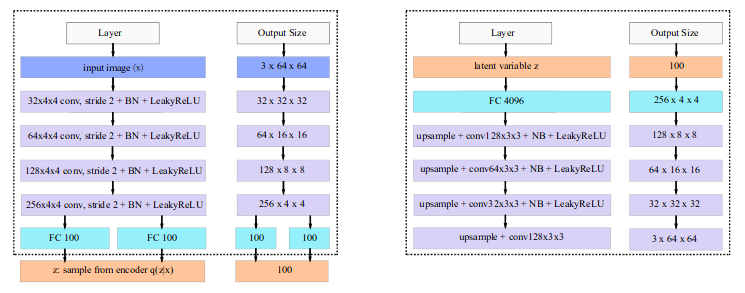
\includegraphics[width=0.9\linewidth]{pictures/detail_arch}}
	\caption{Архитектура сетей автокодировщика}
	\label{fig:detail}
\end{figure}

\section{Результаты и детали обучения}

Был проводен эксперимент на изображениях лиц, чтобы проверить метод. В частности, сначала оцениваем производительность генерации изображения и сравниваем с другими генеративными моделями. Кроме того, мы также исследуем скрытое пространство и изучаем семантические отношения между различными скрытыми представлениями и применяем их для прогнозирования характеристик лица.

Модель была обучена на наборе данных CelebFaces Attributes (CelebA). CelebA - это крупномасштабный набор данных атрибутов лица с 202599 изображениями лиц. Набор обучающих данных путем обрезки и масштабирования выровненных изображений до размера $64 \times 64$ пикселя. Мы обучаем нашу модель с batch size равным  64 для 5 эпох по набору для обучения и используем метод Adam для оптимизации с начальной скоростью обучения 0,0005, которая уменьшается в 0,5 раза для последующих эпох. 19-слойная сеть VGGNet выбрана в качестве сети потерь $\Phi$ для построения потери восприятия функции для восстановления изображения.
Были проведены эксперименты с различными комбинациями слоев, чтобы построить пространственную функцию потерь признаков. Соответственно были обучены две модели: VAE-123 и VAE-345, используя слои relu1\_1, relu2\_1, relu3\_1 и relu3\_1, relu4\_1, relu5\_1 соответственно. Кроме того, размер скрытого вектора $z$ установлен равным 100, как DCGAN, а весовые параметры потерь $\alpha$ и $\beta$ равны 1 и 0,5 соответственно. Реализация была выполнена во фреймворке TensorFlow.

Результаты обучения разделены на две части: реконструкция лица энкодером и декодером, генерация лица из $\mathcal{N}(0, 1)$ декодером и представлены на рисунках \ref{fig:res_autenc_8} и \ref{fig:res_autenc_100}.

\begin{figure}[H]
	\centering
	\captionsetup{justification=centering}
	\subfigure[Оригинальные изображения лиц]{\label{fig:res_autenc_8_1}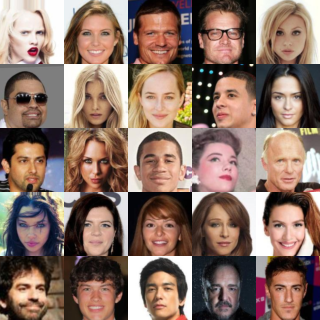
\includegraphics[width=0.3\linewidth]{pictures/9_62000_original_8}} 
	\subfigure[Реконструкция изображений лиц]{\label{fig:res_autenc_8_2}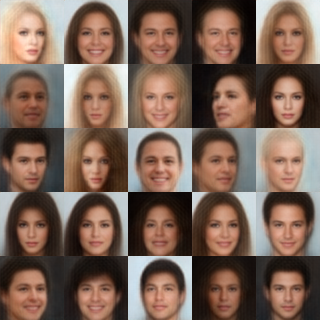
\includegraphics[width=0.3\linewidth]{pictures/9_62000_generated_8}} %\label{fig:4_2}
	\subfigure[Случайная генерация лиц декодером]{\label{fig:res_autenc_8_3}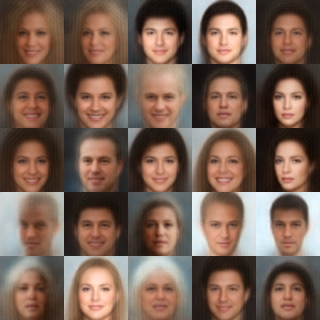
\includegraphics[width=0.3\linewidth]{pictures/9_62000_random_8}} %\label{fig:4_3}
	\caption{Результаты обучения вариационного автокодировщика (размер скрытого вектора 8)}
	\label{fig:res_autenc_8}
\end{figure}

\begin{figure}[H]
	\centering
	\subfigure[Оригинальные изображения лиц]{\label{fig:res_autenc__100_1}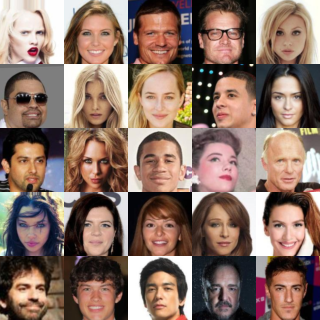
\includegraphics[width=0.3\linewidth]{pictures/9_62000_original_100}} 
	\subfigure[Реконструкция изображений лиц]{\label{fig:res_autenc_100_2}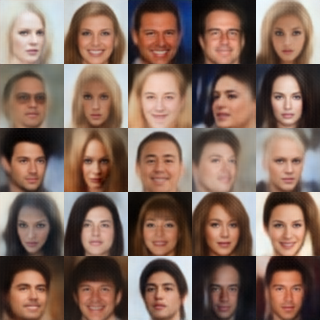
\includegraphics[width=0.3\linewidth]{pictures/9_62000_generated_100}} %\label{fig:4_2}
	\subfigure[Случайная генерация лиц декодером]{\label{fig:res_autenc_100_3}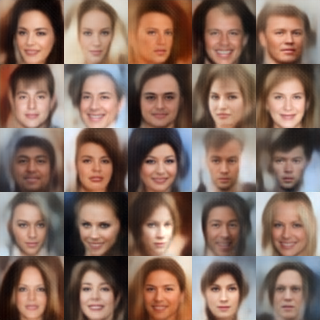
\includegraphics[width=0.3\linewidth]{pictures/9_62000_random_100}} %\label{fig:4_3}
	\caption{Результаты обучения вариационного автокодировщика (размер скрытого вектора 100)}
	\label{fig:res_autenc_100}
\end{figure}


\chapter{Гауссовский процесс и байесовская оптимизация}
\section{Гауссовский процесс}
В настоящее время одним из наиболее популярных методов решения проблемы восстановления (аппроксимации) неизвестной функции путем выборки ее значений является регрессия, основанная на гауссовских процессах.

В рамках этого подхода предполагается, что аппроксимируемая функция является реализацией гауссовского процесса, распределение которого полностью определяется заданной функцией мат. ожидания и функцией дисперсии. Считается, что функция дисперсии между значениями гауссовского процесса зависит только от точек, в которых эти значения получены. Тогда в качестве прогноза, значения аппроксимируемой функции в новой точке используют апостериорное значение мат. ожидания, а для оценки неопределенности этого прогноза - соответствующую апостериорную дисперсию. При этом апостериорное мат. ожидание и апостериорную дисперсию. можно рассчитать аналитически и полностью определить функцией гауссовского процесса.

Обычно предполагается, что функция гауссовского процесса принадлежит некоторому параметрическому семейству, и поэтому задача построения регрессии на основе гауссовских процессов сводится к проблеме оценки параметров самой функции гауссовских процессов.\cite{gauss_proc}

Стандартные методы, основанные на гауссовских процессах, имеют кубическую сложность размера выборки, что делает невозможным их использование в задачах с большими объемами данных. В связи с этим, начиная с 2000-х годов, многие исследователи разрабатывают приблизительные схемы для обучения моделям гауссовских процессов. Развитие методов, основанных на вспомогательных точках (индуцирующих входных данных), позволило применить гауссовские процессы к задачам с большими выборками (более 100 000 объектов).

Гауссовские процессы определяют априорное распределение по набору функций и позволяют находить сложные взаимосвязи в данных. На основе гауссовских процессов было построено много моделей, которые успешно используются для решения различных задач машинного обучения - регрессии и классификации. Эти методы позволяют автоматически корректировать сложность модели, а также позволяют оценить неопределенность в прогнозе.

Таким образом, гауссовский процесс называется случайным процессом, чьи конечномерные распределения гауссовские.

$$
 p(\xi(\omega, x_1), \dots, \xi(\omega,  x_n)) = \mathcal{N}(\xi \arrowvert \mu,  \Sigma)
$$

На рисунке \ref{fig:gauss_process} приводится пример гауссовского процесса. Голубая область показывает $3 \sigma$ - интервал неопределённости процесса (доверительный интервал), а темно-синяя линия — мат. ожидание процесса. Цветные линии показывают случайные реализации процесса.

\begin{figure}[H]
	\center{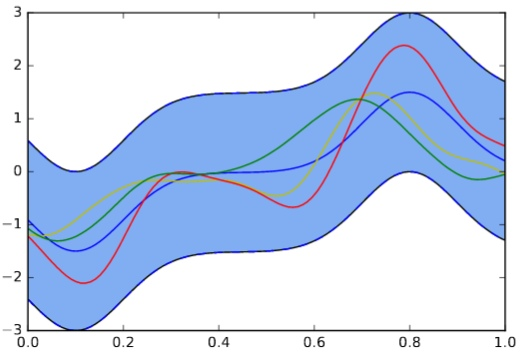
\includegraphics[width=0.7\linewidth]{pictures/gauss_process}}
	\caption{Одномерный гауссовский процесс}
	\label{fig:gauss_process}
\end{figure}

В данной главе рассмотрим гауссовские процессы, заданные на вещественных пространствах $\mathbb{R}^D$ . Тогда случайный процесс называется гауссовским процессом, если для любого $n$, и для любого набора $t_1, t_2, \dots , t_n \in \mathbb{R}^D$ совместное распределение имеет вид.
$$
 f(t_1), f(t_2), \dots, f(t_n) \sim \mathcal{N}(m_t, K_t)
 \text{, где } m_t \in \mathbb{R}^n \text{, } K_t \in \mathbb{R}^{n \times n}
$$

Математическое ожидание определяется функцией среднего $m: \mathbb{R}^D \rightarrow \mathbb{R}$ гауссовского процесса:
$$
 m_t = (m(t_1),  m(t_2),  \dots, m(t_n))^{\top}
$$

Данная функция может быть произвольной.

Аналогично, матрица ковариации $K_t$ определяется ковариационной (ядровой) функцией процесса $k: \mathbb{R}^D \times \mathbb{R}^D \rightarrow \mathbb{R}$.

$$
 K_t =
 \begin{pmatrix}
 k(t_1, t_1)       & k(t_1, t_2) &  \dots & k(t_1, t_n) \\
 k(t_2, t_1)       & k(t_2, t_2) &  \dots & k(t_2, t_n) \\
 \hdotsfor{4} \\
 k(t_n, t_1)       & k(t_n, t_2) &  \dots & k(t_n, t_n)
 \end{pmatrix}
$$

Матрица ковариации для любого набора значений $t_1,  t_2, \dots, t_n$ должна быть симметричной и неотрицательно определенной.

Гауссовский процесс полностью определяется своими функцией математического ожидания и ковариационной функцией. Для гауссовского процесса будем использовать запись:

$$
 f \sim \mathcal{GP}(m(\cdot), k(\cdot, \cdot))
$$
с функиец среднего $m$ и ядровой функцией $k$.

Гауссовские процессы являются довольно гибким средством описания данных, а степень  “гладкости” процесса определяется видом ковариационной функции. На рисунке \ref{fig:dif_gauss_process} представлены примеры реализаций стационарных гауссовских случайных процессов с различными ковариационными функциями.


\begin{figure}[H]
	\captionsetup{justification=centering}
	\center{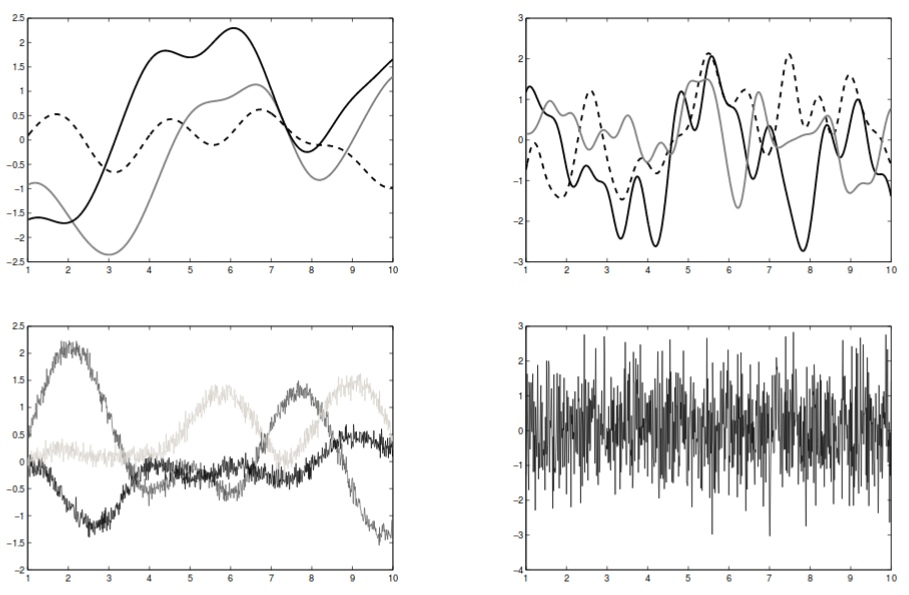
\includegraphics[width=0.7\linewidth]{pictures/dif_gauss_process}}
	\caption{Реализаций стационарных гауссовских случайных процессов с различными ковариационными функциями}
	\label{fig:dif_gauss_process}
\end{figure}

Рассмотрим регрисионную модель на основе гауссовских процессов. Пусть $X=(x_1,  x_2, \dots, x_n)^\top \in \mathbb{R}^{n \times D}$ - описание выборки из n объектов. Пусть $Y=(y_1,  y_2, \dots, y_n)^\top \in \mathbb{R}^{n}$ - соответствующие им значения. Будем считать, что наблюдаемые переменные $y$ - зашумленные значения некоторого скрытого гауссовского процесса $f: \mathbb{R}^D \rightarrow \mathbb{R}$, с нулевым математическим ожиданием и ковариационной функцией $k(\cdot, \cdot)$.

$$
f \sim \mathcal{GP}(0, k(\cdot, \cdot))
$$

Введем скрытые переменные $f = (f_1, f_2, \dots, f_n) \in \mathbb{R}^n$ значения процесса f в точках обучающей выборки. Тогда

$$
 p(y_i \arrowvert f_i) = \mathcal{N}(y_i \arrowvert f_i, \nu^2)
$$
где $\nu$ -- разброс шума. Требуется оценить неизвестное значение процесса $f_{*} \in \mathbb{R}^l$ в наборе новых точек $X_{*} \in \mathbb{R}^{l \times D}$. Рассмотрим модель:

\begin{equation}
 p(y, f \arrowvert X) = p(y \arrowvert 	f) p(f \arrowvert X) = p(f \arrowvert X) \prod\limits_{i=1}^{n} p(y_i \arrowvert f_i)
\end{equation}

Графическая модель для данной задачи изображена на рисунок \ref{fig:gauss_graph_model}.

\begin{figure}[H]
	\captionsetup{justification=centering}
	\center{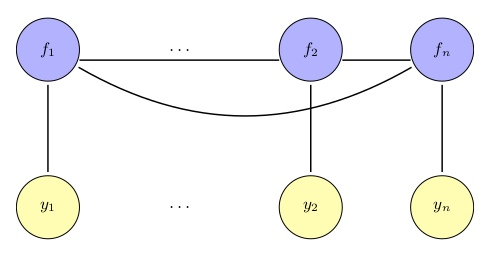
\includegraphics[width=0.7\linewidth]{pictures/gauss_graph_model}}
	\caption{Графическая модель для модели регрессии на основе гауссовских процессов}
	\label{fig:gauss_graph_model}
\end{figure}

Обозначим матрицу попарных значений ковариационной функции, вычисленную на двух наборах точек $A = (a_1, a_2, \dots, a_n)^\top \in \mathbb{R}^{n \times D}$ и $B = (b_1, b_2, \dots, b_m)^\top \in \mathbb{R}^{m \times D}$ как:
$$
  K(A, B) =
 \begin{pmatrix}
 k(a_1, b_1)       & k(a_1, b_2) &  \dots & k(a_1, b_m) \\
 k(a_2, b_1)       & k(a_2, b_2) &  \dots & k(a_2, b_m) \\
 \hdotsfor{4} \\
 k(a_n, b_1)       & k(a_n, b_2) &  \dots & k(a_n, b_m)
 \end{pmatrix}
 \in \mathbb{R}^{n \times m}
$$

Тогда по определению гауссовского процесса распределение

$$
\begin{bmatrix}
f      \\
f_*     \\
\end{bmatrix}
\sim
\mathcal{N} 
\Bigg (0, 
\begin{bmatrix}
K(X,  X) & K(X, X_*) \\
K(X_*,  X) & K(X_*, X_*) \\
\end{bmatrix}
\Bigg )
$$

Так как $y$ представляет из себя зашумленную версию $f$ , то

$$
\begin{bmatrix}
y      \\
f_*     \\
\end{bmatrix}
\sim
\mathcal{N} 
\Bigg (0, 
\begin{bmatrix}
K(X,  X) + \nu^2 I & K(X, X_*) \\
K(X_*,  X) & K(X_*, X_*) \\
\end{bmatrix}
\Bigg )
$$

Можем выразить условное распределение на $f_*$ при условии данных

$$
 f_* \arrowvert y \sim \mathcal{N}(\hat{m}, \hat{K})
$$
где

\begin{equation} 
	\begin{array}{r@{}l} \label{eq:18}
		&{} \mathbb{E} [f_* \arrowvert y] = \hat{m} = K(X_*, X) (K(X, X) + \nu^2 I)^{-1} y\\
		&{} cov(f_* \arrowvert y) = \hat{K} = K(X_*, X_*) - K(X_*,  X) (K(X, X) + \nu^2 I)^{-1} K(X, X_{*}) \\
	\end{array}{}
\end{equation}

Таким образом, сложность получения распределения на $f_*$ определяется сложностью обращения матрицы $K(X, X) + \nu^2 I \in \mathcal{R}^{n \times n}$ и имеет асимптотику $\mathcal{O}(n^3)$.

На рисунке \ref{fig:predict_gauss_proc} показан пример предсказательного распределения для гауссовского процесса с $\nu = 0$, настроенного по трем точкам, обозначенным синими кругами. Голубая область показывает $3\sigma$-интервал для значений процесса, а темно-синяя линия — его математическое ожидание. Цветные линии показывают случайные реализации процесса.

\begin{figure}[H]
	\captionsetup{justification=centering}
	\center{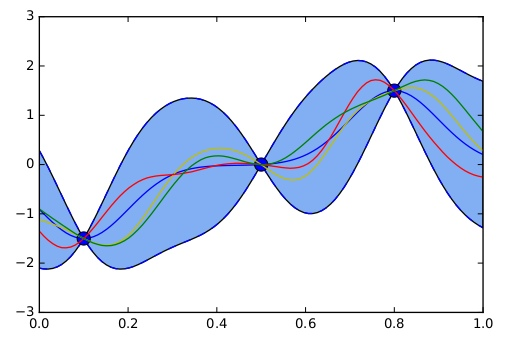
\includegraphics[width=0.7\linewidth]{pictures/predict_gauss_process}}
	\caption{Предсказательное распределение в задаче регрессии}
	\label{fig:predict_gauss_proc}
\end{figure}

\section{Байесовская оптимизация}

Байесовская оптимизация (Bayes Optimization) представляет собой класс методов оптимизации на основе машинного обучения, ориентированных на решение задачи.

\begin{equation} \label{eq:17}
 \max\limits_{x \in A}^{} f(x)
\end{equation}
где допустимое множество и целевая функция обычно имеют следующие свойства:
\begin{itemize}
	\item $x$ находится в $\mathbb{R}^d$, где значени $d$ не слишком велико. Обычно при $d \leq 20$ наиболее успешные приложения байесовской оптимизации,
	\item целевая функция $f$ непрерывна. Обычно это требуется для моделирования $f$ с использованием регрессии на основе гауссовского процесса,
	\item $f$ «дорого вычислять» в том смысле, что число вычислений, которые могут быть выполнены, ограничено, как правило, несколькими сотнями. Это ограничение обычно возникает из-за того, что каждое вычисление значения функции занимает значительное количество времени (обычно часов), но также может происходить из-за того, что данное вычисление может нести денежные затраты (например, от покупки мощности облачных вычислений или покупки лабораторных материалов) или альтернативные затраты (например, если вычисление $f$ требует задавать человеку вопросы, которые будут терпеть только ограниченное число раз),
	\item $f$, по своей природе, не является вогнутой или линейной, хотя данные характеристики позволили бы упростить оптимизацию с использованием известных и класиических методов, которые используют данные свойства для повышения эффективности,
	\item когда происходит вычисление $f$, нет возможности получить никаких производных первого или второго порядка. Это отрицате применение методов оптимизации первого и второго порядка, таких как градиентный спуск, метод Ньютона или квазиньютоновские методов. Проблемы с данным свойством называются «без производных»,
	\item $f(x)$ наблюдается без шума. Однако почти во всех работах по байесовской оптимизации шум считается независимым от вычислений и гауссовым с постоянной дисперсией (обычно стандартное гауссовое распределение),
	\item внимание акцентировано на поиске глобального, а не локального оптимума.
\end{itemize}

Байесовская оптимизация состоит из двух основных компонентов: байесовской статистической модели для моделирования целевой функции (обычно гауссовский процесс) и функции оценки (acquisition function) для принятия решения о том, где искать оптимум дальше. После вычисления целевой функции в соответствии с первоначальными данными, просиходит вычисление Гауссовского процесса и его обучения для подбора параметров функции ковариционной (ядровой) функции. После этого составляется функция оценки на основе полученного Гауссовского процесса, находится оптимум данной функции оценки, вычисляется значение целевой функции в данном оптимуме, после чего данное значение добавляется в набор данных. Процесс повторяется снова до определённой сходимости или после вычисления определённого количества итераций. Всё вышеописанное обобщается в алгоритм.
%Пока не сойдётся (или пока количество итераций не достигнет %определнного числа):

%Статистическая модель, которая всегда является гауссовским процессом, обеспечивает байесовское апостериорное распределение вероятностей, которое описывает потенциальные значения для $f(x)$ в точке-кандидате $x$. Каждый раз, когда мы наблюдаем $f$ в новой точке, это апостериорное распределение обновляется. Функция сбора измеряет значение, которое будет сгенерировано путем оценки целевой функции в новой точке $x$ на основе текущего апостериорного распределения по $f$.

Одна итерация байесовской оптимизации с использованием регрессии гауссовского процесса и функцией оценки ожидаемого улучшения (Expected \\ improvement) проиллюстрирована на рисунке \ref{fig:one_iter_bay_opt}. На верхней панели показаны бесшумные значения целевой функции с синими кружками в трех точках. Он также показывает результат регрессии гауссовского процесса. Регрессия гауссова процесса дает апостериорное распределение вероятностей для каждого $f(x)$, которое обычно распределяется со средним значением $\mu_n(x)$ и дисперсией $\sigma^2_n(x)$. Это изображено на рисунке \ref{fig:one_iter_bay_opt} с $\mu_n(x)$ в виде сплошной красной линии и 95 \% байесовским доверительным интервалом для $f(x)$, $\mu_n(x) \pm 1,96 \times \sigma_n(x)$ в виде пунктирных красных линий. Среднее можно интерпретировать как точечную оценку $f(x)$. Достоверный интервал действует как доверительный интервал в статистике частых случаев и содержит $f(x)$ с вероятностью 95 \% в соответствии с последним распределением. Среднее значение интерполируется ранее данным точкам (начальным данным). В этих точках доверительный интервал имеет ширину 0 и расширяется по мере удаления от них.\cite{bayess}

Нижний рисунок показывает функцию оценки ожидаемого улучшение (Expected improvement) функции сбора, которая соответствует данному  апостериору Гауссовского процесса. Стоит обратить внимание, что она принимает значение 0 в точках, которые были ранее вычислены. Это приемлимо, когда значения целевой функции не имеют шума, потому что они не дают полезной информации для решения. Также стоит обратить внимание, что она имеет тенденцию быть больше для точек с большими доверительными интервалами, потому что значения точки, где Гауссовский процесс более не уверен в цели, имеет тенденцию быть более полезным в поиске хороших приближенных глобальных оптимумов. Стоит обратить внимание, что она имеет тенденцию быть больше для точек с большим апостериорным средним, потому что такие точки, как правило, близки к хорошим приблизительным глобальным оптимумам.
\begin{figure}[H]
	\captionsetup{justification=centering}
	\center{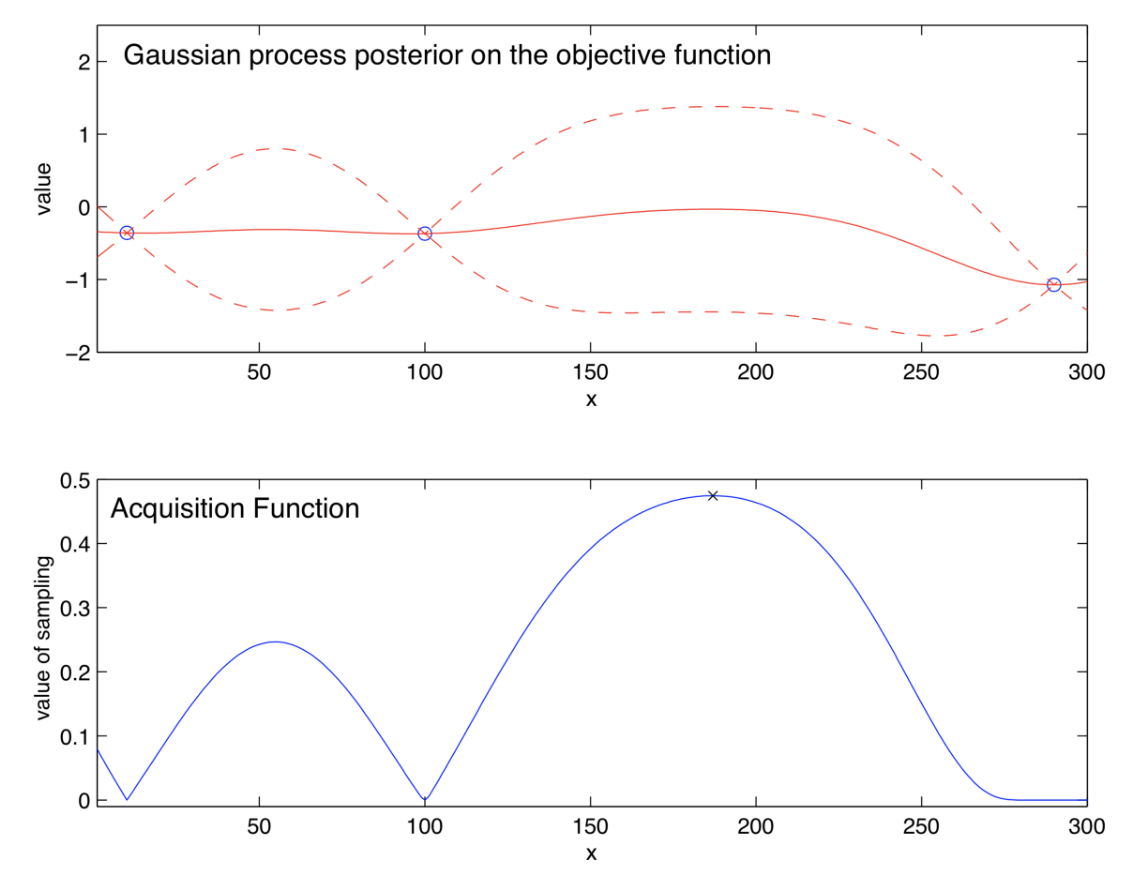
\includegraphics[width=0.9\linewidth]{pictures/one_iter_bay_opt}}
	\caption{Предсказательное распределение в задаче регрессии}
	\label{fig:one_iter_bay_opt}
\end{figure}

Функция оценки ожидаемого улучшение (Expected improvement) выводится из эксперимента. Допустим использование алгоритма байесовской оптимизации для решения \eqref{eq:17}, в котором $x_n$ обозначает точку, выбранную на итерации $n$, а $y_n$ обозначает соответствующее ей значение. Допустим решение как наше окончательное решение \eqref{eq:17}. Также допустим, что нет возможности получить значение функции, которое необходимо, и решение должно быть основано на тех, которые уже выполнены. Поскольку мы вычисляем $f$ без шума, оптимальным решением является предварительно вычисленная точка с наибольшим полученным значением. Пусть $f_n^* = \max_{m \leq n} f(x_m)$ будет значением этой точки, где $n$ - количество итераций.

Теперь предположим, что на самом деле есть возможность выполнить одно дополнительное вычисление, и можно его выполнить где угодно и когда угодно. Если вычислить в $x$, получится значение $f(x)$. После получения нового значения лучшей точки должно быть либо $f(x)$ (если $f(x) \geq f_n^*$), либо $f_n^*$ (если $f(x) \leq f_n^*$). Улучшение $f(x) - f_n^*$ положительное или 0 в противном случае. Тогда данное улучшение можно записать более компактно как $[f(x) - f_n^*]^+$, где $a^+ = \max(a, 0)$. 

Необходимо выбрать $x$, чтобы данное улучшение было большим, так как $f(x)$ неизвестно до окончания вычисления. Однако можно взять мат. ожидание этого улучшения и выбирать $x$, относительно максимизации мат. ожидания. Определяем мат. ожидание как.

$$
 EI_n(x) \coloneqq E_n [[f(x) - f_n^*]^+]
$$

Здесь $E_n[\cdot] = E_n[\cdot \arrowvert x_{1:n}, y_{1:n}]$ указывает мат. ожидание апостериорного распределения, данное при вычислении $f$ в $x_1 , \dots, x_n$. Это апостериорное распределение $f(x)$ задаётся формулой \eqref{eq:18}. 

Ожидаемое улучшение может быть вычислено с помощью формулы интегрирования по частям. Опустив вычисления, получим.
$$
 EI_n(x) = var[\hat{f_n}(x)] (z_n \Phi(z_n) + \Phi(z_n))
$$
где 
\begin{align*}
 z_n &= \frac{\mathbb{E} \hat{f_n}(x)-m(x)}{var[\hat{f_n}(x)]}, \\
 \Phi & \text{ -- функция плотности нормального распределения (функция распределения), } \\
 \hat{f_n} & \text{ -- статистическая модель на $n$-ой итерации (Гауссовский процесс).}
\end{align*}

Затем решается задача оптимизации:

\begin{equation} \label{eq:19}
 x_{n+1} =  \arg\!\max EI_n (x)
\end{equation}

В отличие от целевой функции $f$ в нашей первоначальной задаче оптимизации \eqref{eq:17}, $EI_n(x)$ является недорогой для вычисления и позволяет легко оценить производные первого и второго порядка. Реализации алгоритма ожидаемого улучшения могут также использовать непрерывный методы  оптимизации первого или второго порядка для решения \eqref{eq:19}. Например, один метод, который хорошо зарекомендовал себя для автора, - это вычислить первые производные и использовать квазиньютоновский метод L-BFGS-B (Liu and Nocedal, 1989).

На рисунке \ref{fig:contour_plot_EI} показан график линий уровня $EI_n(x)$ в терминах $\vartriangle_n (x) = \mathbb{E} \hat{f}(x)- m(x)$ и апостериорного стандартного отклонения $\sigma_n (x) = var[\hat{f_n}(x)]$. $EI_n(x)$ увеличивается при увелечении и $\vartriangle_n (x)$, и  $\sigma_n (x)$. Кривые $\vartriangle_n (x)$ и $\sigma_n (x)$ с равным $EI$ показывают, как $EI$ балансирует между оценкой в точках с высоким ожидаемым улучшением (высоким $\vartriangle_n (x)$)) и высокой неопределенностью (высоким $\sigma_n (x)$). В контексте оптимизации вычисление в точках с высоким ожидаемым улучшением относительно предыдущей наилучшей точки является наиболее важные, потому что хорошие приблизительные глобальные оптимумы, вероятно, будут находиться около таких точек. С другой стороны, вычисление в точках с высокой неопределенностью перспективна, потому что поиск оптимума просихожит в тех местах, о которых мало известно Гауссовскому процессу (высокий разброс значений) и которые, как правило, находятся далеко от того, что ранне было вычислено. Оптимум, который может быть значительно лучше, чем тот, которую уже есть, вполне возможно может быть в тех местах. \cite{bayess}

\begin{figure}[H]
	\captionsetup{justification=centering}
	\center{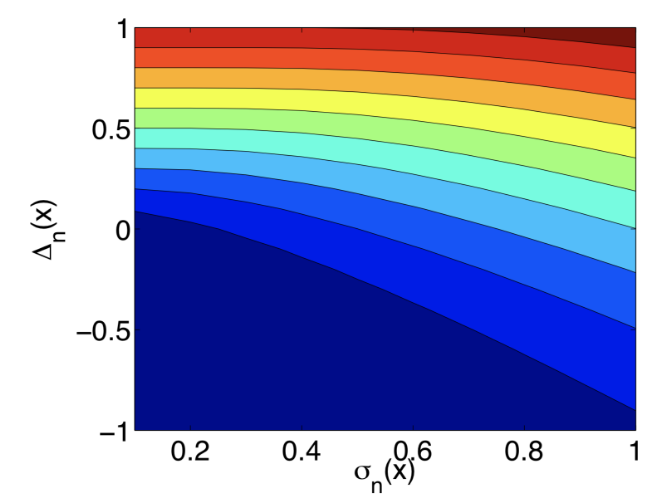
\includegraphics[width=0.6\linewidth]{pictures/contour_plot_EI}}
	\caption{График линий уровня $EI(x)$}
	\label{fig:contour_plot_EI}
\end{figure}

Рисунок \ref{fig:one_iter_bay_opt} показывается $EI(х)$ на нижнем графике. Можно отследить поведение данной функции, где наибольшее ожидаемое улучшение, ищется там, где высокое стандартное отклонение (далеко от ранее вычисленных точек) и высокое мат. ожидание. Наименьшее ожидаемое улучшение - 0 в точках, где известны значения целевой функции. Стандартное отклонение в этих точках равны 0, а мат. ожидание обязательно не больше, чем лучшая ранее вычисленный оптимум.

В данной работе было предложено подстраивать значения скрытого вектора $z$ декодера автокодировщика под генерацию лица наперёд заданным визуальным характеристикам при помощи Байесовской оптимизации. Задача пользователя заключается в оценивании списка сгенерированных (по определённым скрытым векторам) лиц по 5-бальной шкале по заданной характеристике (больше-лучше). Затем байесовская оптимизация пытается предложить наиболее лучший скрытый вектор $z$ (необязательно из существующих в списке сгенерированных, но он может быть очень похож на один из существующих), которые отправляется в декодер автокодировщике и из этого вектора декодируется лицо с наиболее лучшей визуальной характеристикой. Целевая функция для данного типа оптимизации задавалась как $\frac{\text{mark}}{\max(\text{mark})}$. Веса модели автокодировщика взяты с размером скрытого вектор равного 8. Результаты представлены на рисунках \ref{fig:res_bay_opt_hair} и \ref{fig:res_bay_opt_smile}.

\begin{figure}[H]
	\centering
	\captionsetup{justification=centering}
	\subfigure[Список сгенерированных лиц и их оценки ]{\label{fig:res_bay_opt_hair_1}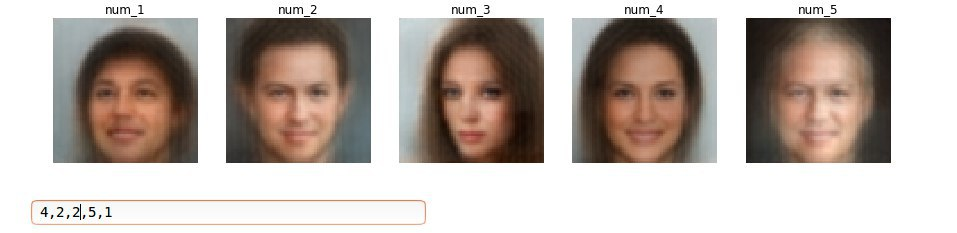
\includegraphics[width=0.7\linewidth]{pictures/bay_opt_dark_hair}} \\
	\subfigure[Результат выбора лица с наиболее тёмными волосами ]{\label{fig:res_bay_opt_hair_2}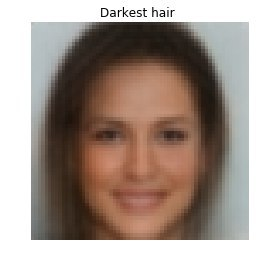
\includegraphics[width=0.2\linewidth]{pictures/bay_opt_darkest_hair}} 
	\caption{Результат применения Байесовской оптимизации к подбору значений скрытого вектора декодера автокодировщика для характеристики наиболее тёмных волос.}
	\label{fig:res_bay_opt_hair}
\end{figure}

\begin{figure}[H]
	\centering
	\captionsetup{justification=centering}
	\subfigure[Список сгенерированных лиц и их оценки]{\label{fig:res_bay_opt_smile_1}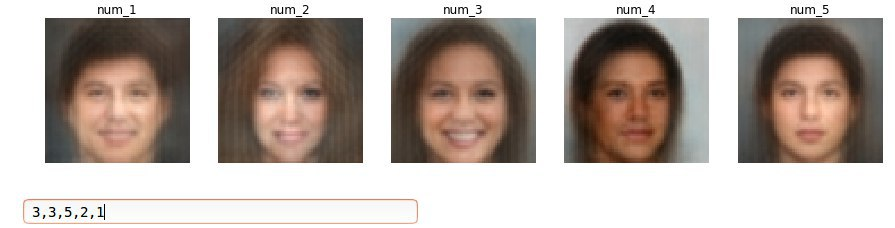
\includegraphics[width=0.7\linewidth]{pictures/bay_opt_wide_smile}} \\
	\subfigure[Результат выбора лица с наиболее широкой улыбкой ]{\label{fig:res_bay_opt_smile_2}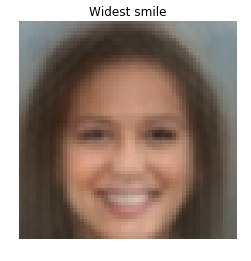
\includegraphics[width=0.2\linewidth]{pictures/bay_opt_widest_smile}} 
	\caption{Результат применения Байесовской оптимизации к подбору значений скрытого вектора декодера автокодировщика для характеристики наиболее широкой улыбки.}
	\label{fig:res_bay_opt_smile}
\end{figure}







